\documentclass{article}
\usepackage{tikz}
\usetikzlibrary{external}
\tikzexternalize[prefix=figures/]
\usepackage{latexml}
\iflatexml
\tikzset{external/system call={echo "\texsource" | latexml --nocomments --quiet --quiet --destination "\image.xml" --documentid="\image" -}}
% \texsource becomes \def\tikzexternalrealjob{exttest}\documentclass{article}
\usepackage{tikz}
\usetikzlibrary{external}
\tikzexternalize[prefix=figures/]
\usepackage{latexml}
\iflatexml
\tikzset{external/system call={echo "\texsource" | latexml --nocomments --quiet --quiet --destination "\image.xml" --documentid="\image" -}}
% \texsource becomes \def\tikzexternalrealjob{exttest}\documentclass{article}
\usepackage{tikz}
\usetikzlibrary{external}
\tikzexternalize[prefix=figures/]
\usepackage{latexml}
\iflatexml
\tikzset{external/system call={echo "\texsource" | latexml --nocomments --quiet --quiet --destination "\image.xml" --documentid="\image" -}}
% \texsource becomes \def\tikzexternalrealjob{exttest}\documentclass{article}
\usepackage{tikz}
\usetikzlibrary{external}
\tikzexternalize[prefix=figures/]
\usepackage{latexml}
\iflatexml
\tikzset{external/system call={echo "\texsource" | latexml --nocomments --quiet --quiet --destination "\image.xml" --documentid="\image" -}}
% \texsource becomes \def\tikzexternalrealjob{exttest}\input{exttest}
% standard is
% pdflatex -shell-escape -halt-on-error -interaction=batchmode -jobname "\image" "\texsource"
\typeout{doc id is \lxGetDocumentID}
\fi
\usepackage{custom}
\typeout{jobname is \jobname}
%\newcommand{\exttestnextfilename}{}
%\tikzexternalgetnextfilename\exttestnextfilename
%\typeout{next file name is \exttestnextfilename}
\makeatletter
%\tikzexternal@getnextfilename\exttestnextfilename
%\typeout{next at file name is \exttestnextfilename}
\typeout{tikzexternal@curfilename is \tikzexternal@curfilename}
%\show\tikzexternal@curfilename
\makeatother
\typeout{pgfactualjobname is \pgfactualjobname}
% in LaTeXML regular:
%jobname is exttest
%tikzexternal@curfilename is \tikzexternal@curfilename
%pgfactualjobname is exttest
% in TeX regular:
%jobname is exttest
%tikzexternal@curfilename is \tikzexternal@curfilename 
%pgfactualjobname is exttest
% in LaTeXML system call:
%jobname is exttest
%tikzexternal@curfilename is \tikzexternal@curfilename
%pgfactualjobname is Anonymous String
% in TeX system call:
%jobname is figures/exttest-figure0
%tikzexternal@curfilename is \tikzexternal@curfilename 
%pgfactualjobname is figures/exttest-figure0
%\show\pgfrealjobname
\begin{document}
A small document.
\tikzset{external/remake next}
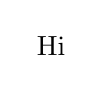
\begin{tikzpicture}
\node(1,1){Hi};
\end{tikzpicture}
Done.
\end{document}

%/Users/tprescott/Library/texmf/tex/generic/pgf/frontendlayer/tikz/libraries/tikzexternalshared.code.tex 

% L699
% L811

% standard is
% pdflatex -shell-escape -halt-on-error -interaction=batchmode -jobname "\image" "\texsource"
\typeout{doc id is \lxGetDocumentID}
\fi
\usepackage{custom}
\typeout{jobname is \jobname}
%\newcommand{\exttestnextfilename}{}
%\tikzexternalgetnextfilename\exttestnextfilename
%\typeout{next file name is \exttestnextfilename}
\makeatletter
%\tikzexternal@getnextfilename\exttestnextfilename
%\typeout{next at file name is \exttestnextfilename}
\typeout{tikzexternal@curfilename is \tikzexternal@curfilename}
%\show\tikzexternal@curfilename
\makeatother
\typeout{pgfactualjobname is \pgfactualjobname}
% in LaTeXML regular:
%jobname is exttest
%tikzexternal@curfilename is \tikzexternal@curfilename
%pgfactualjobname is exttest
% in TeX regular:
%jobname is exttest
%tikzexternal@curfilename is \tikzexternal@curfilename 
%pgfactualjobname is exttest
% in LaTeXML system call:
%jobname is exttest
%tikzexternal@curfilename is \tikzexternal@curfilename
%pgfactualjobname is Anonymous String
% in TeX system call:
%jobname is figures/exttest-figure0
%tikzexternal@curfilename is \tikzexternal@curfilename 
%pgfactualjobname is figures/exttest-figure0
%\show\pgfrealjobname
\begin{document}
A small document.
\tikzset{external/remake next}
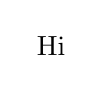
\begin{tikzpicture}
\node(1,1){Hi};
\end{tikzpicture}
Done.
\end{document}

%/Users/tprescott/Library/texmf/tex/generic/pgf/frontendlayer/tikz/libraries/tikzexternalshared.code.tex 

% L699
% L811

% standard is
% pdflatex -shell-escape -halt-on-error -interaction=batchmode -jobname "\image" "\texsource"
\typeout{doc id is \lxGetDocumentID}
\fi
\usepackage{custom}
\typeout{jobname is \jobname}
%\newcommand{\exttestnextfilename}{}
%\tikzexternalgetnextfilename\exttestnextfilename
%\typeout{next file name is \exttestnextfilename}
\makeatletter
%\tikzexternal@getnextfilename\exttestnextfilename
%\typeout{next at file name is \exttestnextfilename}
\typeout{tikzexternal@curfilename is \tikzexternal@curfilename}
%\show\tikzexternal@curfilename
\makeatother
\typeout{pgfactualjobname is \pgfactualjobname}
% in LaTeXML regular:
%jobname is exttest
%tikzexternal@curfilename is \tikzexternal@curfilename
%pgfactualjobname is exttest
% in TeX regular:
%jobname is exttest
%tikzexternal@curfilename is \tikzexternal@curfilename 
%pgfactualjobname is exttest
% in LaTeXML system call:
%jobname is exttest
%tikzexternal@curfilename is \tikzexternal@curfilename
%pgfactualjobname is Anonymous String
% in TeX system call:
%jobname is figures/exttest-figure0
%tikzexternal@curfilename is \tikzexternal@curfilename 
%pgfactualjobname is figures/exttest-figure0
%\show\pgfrealjobname
\begin{document}
A small document.
\tikzset{external/remake next}
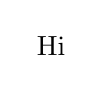
\begin{tikzpicture}
\node(1,1){Hi};
\end{tikzpicture}
Done.
\end{document}

%/Users/tprescott/Library/texmf/tex/generic/pgf/frontendlayer/tikz/libraries/tikzexternalshared.code.tex 

% L699
% L811

% standard is
% pdflatex -shell-escape -halt-on-error -interaction=batchmode -jobname "\image" "\texsource"
\typeout{doc id is \lxGetDocumentID}
\fi
\usepackage{custom}
\typeout{jobname is \jobname}
%\newcommand{\exttestnextfilename}{}
%\tikzexternalgetnextfilename\exttestnextfilename
%\typeout{next file name is \exttestnextfilename}
\makeatletter
%\tikzexternal@getnextfilename\exttestnextfilename
%\typeout{next at file name is \exttestnextfilename}
\typeout{tikzexternal@curfilename is \tikzexternal@curfilename}
%\show\tikzexternal@curfilename
\makeatother
\typeout{pgfactualjobname is \pgfactualjobname}
% in LaTeXML regular:
%jobname is exttest
%tikzexternal@curfilename is \tikzexternal@curfilename
%pgfactualjobname is exttest
% in TeX regular:
%jobname is exttest
%tikzexternal@curfilename is \tikzexternal@curfilename 
%pgfactualjobname is exttest
% in LaTeXML system call:
%jobname is exttest
%tikzexternal@curfilename is \tikzexternal@curfilename
%pgfactualjobname is Anonymous String
% in TeX system call:
%jobname is figures/exttest-figure0
%tikzexternal@curfilename is \tikzexternal@curfilename 
%pgfactualjobname is figures/exttest-figure0
%\show\pgfrealjobname
\begin{document}
A small document.
\tikzset{external/remake next}
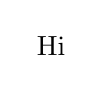
\begin{tikzpicture}
\node(1,1){Hi};
\end{tikzpicture}
Done.
\end{document}

%/Users/tprescott/Library/texmf/tex/generic/pgf/frontendlayer/tikz/libraries/tikzexternalshared.code.tex 

% L699
% L811
